\documentclass[tikz,14pt,border=10pt]{standalone}
\usepackage[utf8]{inputenc}
\usepackage{tikz}
\usetikzlibrary{shapes.geometric, arrows}

\tikzstyle{var} = [circle, minimum width=1cm, minimum height=1cm,text centered, draw=black]
\tikzstyle{arrow} = [thick,->,>=stealth]

\begin{document}

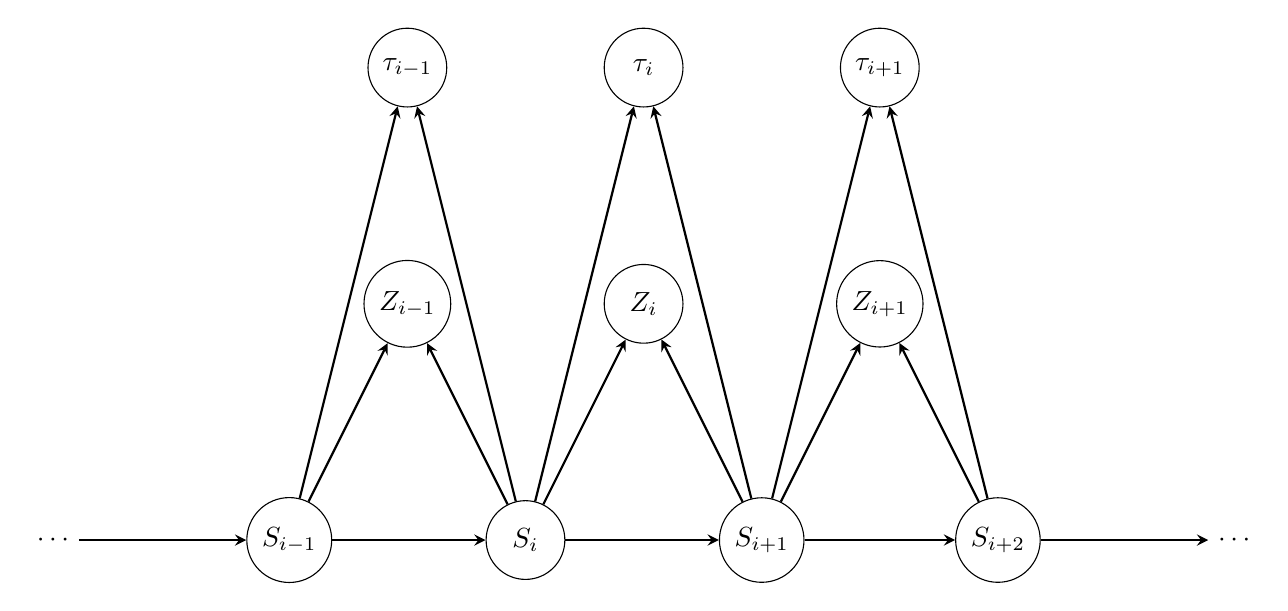
\begin{tikzpicture}[node distance=3cm]
\node (left_ellipse) []{$\cdots$};

\node (Sm1) [var, right of=left_ellipse] {$S_{i-1}$};
\node (Zm1) [var, above of=Sm1, xshift=1.5cm] {$Z_{i-1}$};
\node (tm1) [var, above of=Zm1] {$\tau_{i-1}$};


\node (S) [var, right of=Sm1] {$S_{i}$};
\node (Z) [var, right of=Zm1] {$Z_{i}$};
\node (t) [var, above of=Z] {$\tau_{i}$};

\node (Sp1) [var, right of=S] {$S_{i+1}$};
\node (Zp1) [var, right of=Z] {$Z_{i+1}$};
\node (tp1) [var, above of=Zp1] {$\tau_{i+1}$};


\node (Sp2) [var, right of=Sp1] {$S_{i+2}$};
%\node (Zp2) [var, right of=Z] {$Z_{i+2}$};
%\node (tp2) [var, below of=Sp2] {$\tau_{i+2}$};

\node (right_ellipse) [right of=Sp2]{$\cdots$};

\draw [arrow] (left_ellipse) -- (Sm1);
\draw [arrow] (Sm1) -- (Zm1);
\draw [arrow] (Sm1) -- (tm1);
\draw [arrow] (Sm1) -- (S);
\draw [arrow] (S) -- (Z);
\draw [arrow] (S) -- (t);
\draw [arrow] (S) -- (Sp1);
\draw [arrow] (S) -- (Zm1);
\draw [arrow] (S) -- (tm1);
\draw [arrow] (Sp1) -- (Zp1);
\draw [arrow] (Sp1) -- (tp1);
\draw [arrow] (Sp1) -- (Sp2);
\draw [arrow] (Sp1) -- (Z);
\draw [arrow] (Sp1) -- (t);
%\draw [arrow] (Sp2) -- (Zp2);
%\draw [arrow] (Sp2) -- (tp2);
%\draw [arrow] (Sp2) -- (Zp2);
\draw [arrow] (Sp2) -- (Zp1);
\draw [arrow] (Sp2) -- (tp1);
\draw [arrow] (Sp2) -- (right_ellipse);

%\node (in1) [io, below of=start] {Input};
%\node (pro1) [process, below of=in1] {Process 1};
%\node (dec1) [decision, below of=pro1, yshift=-0.5cm] {Decision 1};
%\node (pro2a) [process, below of=dec1, yshift=-0.5cm] {Process 2a text text text text text text text text text text};
%\node (pro2b) [process, right of=dec1, xshift=2cm] {Process 2b};
%\node (out1) [io, below of=pro2a] {Output};
%\node (stop) [startstop, below of=out1] {Stop};
%
%\draw [arrow] (start) -- (in1);
%\draw [arrow] (in1) -- (pro1);
%\draw [arrow] (pro1) -- (dec1);
%\draw [arrow] (dec1) -- node[anchor=east] {yes} (pro2a);
%\draw [arrow] (dec1) -- node[anchor=south] {no} (pro2b);
%\draw [arrow] (pro2b) |- (pro1);
%\draw [arrow] (pro2a) -- (out1);
%\draw [arrow] (out1) -- (stop);


\end{tikzpicture}

\end{document}